\documentclass{beamer}
%
% Choose how your presentation looks.
%
% For more themes, color themes and font themes, see:
% http://deic.uab.es/~iblanes/beamer_gallery/index_by_theme.html
%
\mode<presentation>
{
  \usetheme{Madrid}      % or try Darmstadt, Madrid, Warsaw, ...
  \usecolortheme{whale} % or try albatross, beaver, crane, ...
  \usefonttheme{professionalfonts}  % or try serif, structurebold, ...
  \setbeamertemplate{navigation symbols}{}
  \setbeamertemplate{caption}[numbered]
} 

\usepackage[english]{babel}
\usepackage[utf8x]{inputenc}
\usepackage{multirow}
\usepackage{graphicx}
\usepackage[export]{adjustbox}
\usepackage{subcaption}
\usepackage[labelfont=scriptsize, textfont=scriptsize]{subcaption}
\newcommand*\dif{\mathop{}\!\mathrm{d}}



\title[Machine Learning and NLSE]{Machine Learning and Non-linear Schrödinger Equation}
\author{Hüseyin Talha Şenyaşa}
\institute{Graduation Project}
%\date{\today}

\begin{document}

\begin{frame}
  \titlepage
\end{frame}

% Uncomment these lines for an automatically generated outline.
\begin{frame}{Outline}
  \tableofcontents
\end{frame}

\section{Gross-Pitaevskii Equation in Random 1D Potentials}

%\begin{frame}{Gross-Pitaevskii Equation}
%
%$\bullet$ Bose-Einstein Condensate at zero temperature
%
%$$\hat{H} = \sum_{i = 1}^{N} \left(\frac{\boldsymbol{p}_i^2}{2m} + V(\boldsymbol{r}_i) \right) + %\frac{1}{2} \sum_{i = 1}^{N} \sum_{j \neq i}^{N} U(|\boldsymbol{r}_i - \boldsymbol{r}_j|)$$
%
%$$-\alpha\frac{d^2\widetilde{\psi}}{d\widetilde{x}^2} + \widetilde{V}(\widetilde{x})\widetilde{\psi} %+ \widetilde{g}|\widetilde{\psi}|^2 \widetilde{\psi} = \widetilde{\mu}\widetilde{\psi} $$
%
%$\bullet$ $g|\psi|^2$ term introduces non-linearty. (Interactions between bosons)
%\vskip 0.5cm
%
%$\bullet$ Analytic solutions are known for only few cases.
%\vskip 0.5cm
%
%$\bullet$ Generally solved by numerically or by approximation.
%    
%\end{frame}

\begin{frame}{Gross-Pitaevskii Equation in Random 1D Potentials}

$\bullet$ Bose-Einstein Condensate at zero temperature
\vskip 0.3cm

$\bullet$ $\frac{-\hbar^2}{2m}\frac{\dif^2\psi_x}{\dif x^2} + V(x)\psi + g_{1\text{D}}|\psi|^2\psi = \mu_{1\text{D}}\psi $
\vskip 0.3cm

$\bullet$ $g|\psi|^2$ term introduces non-linearty. (Interactions between bosons)
\vskip 0.3cm

$\bullet$ Numerically solved in XMDS Framework.
\vskip 0.3cm


\begin{columns}
\begin{column}{0.8\textwidth}
    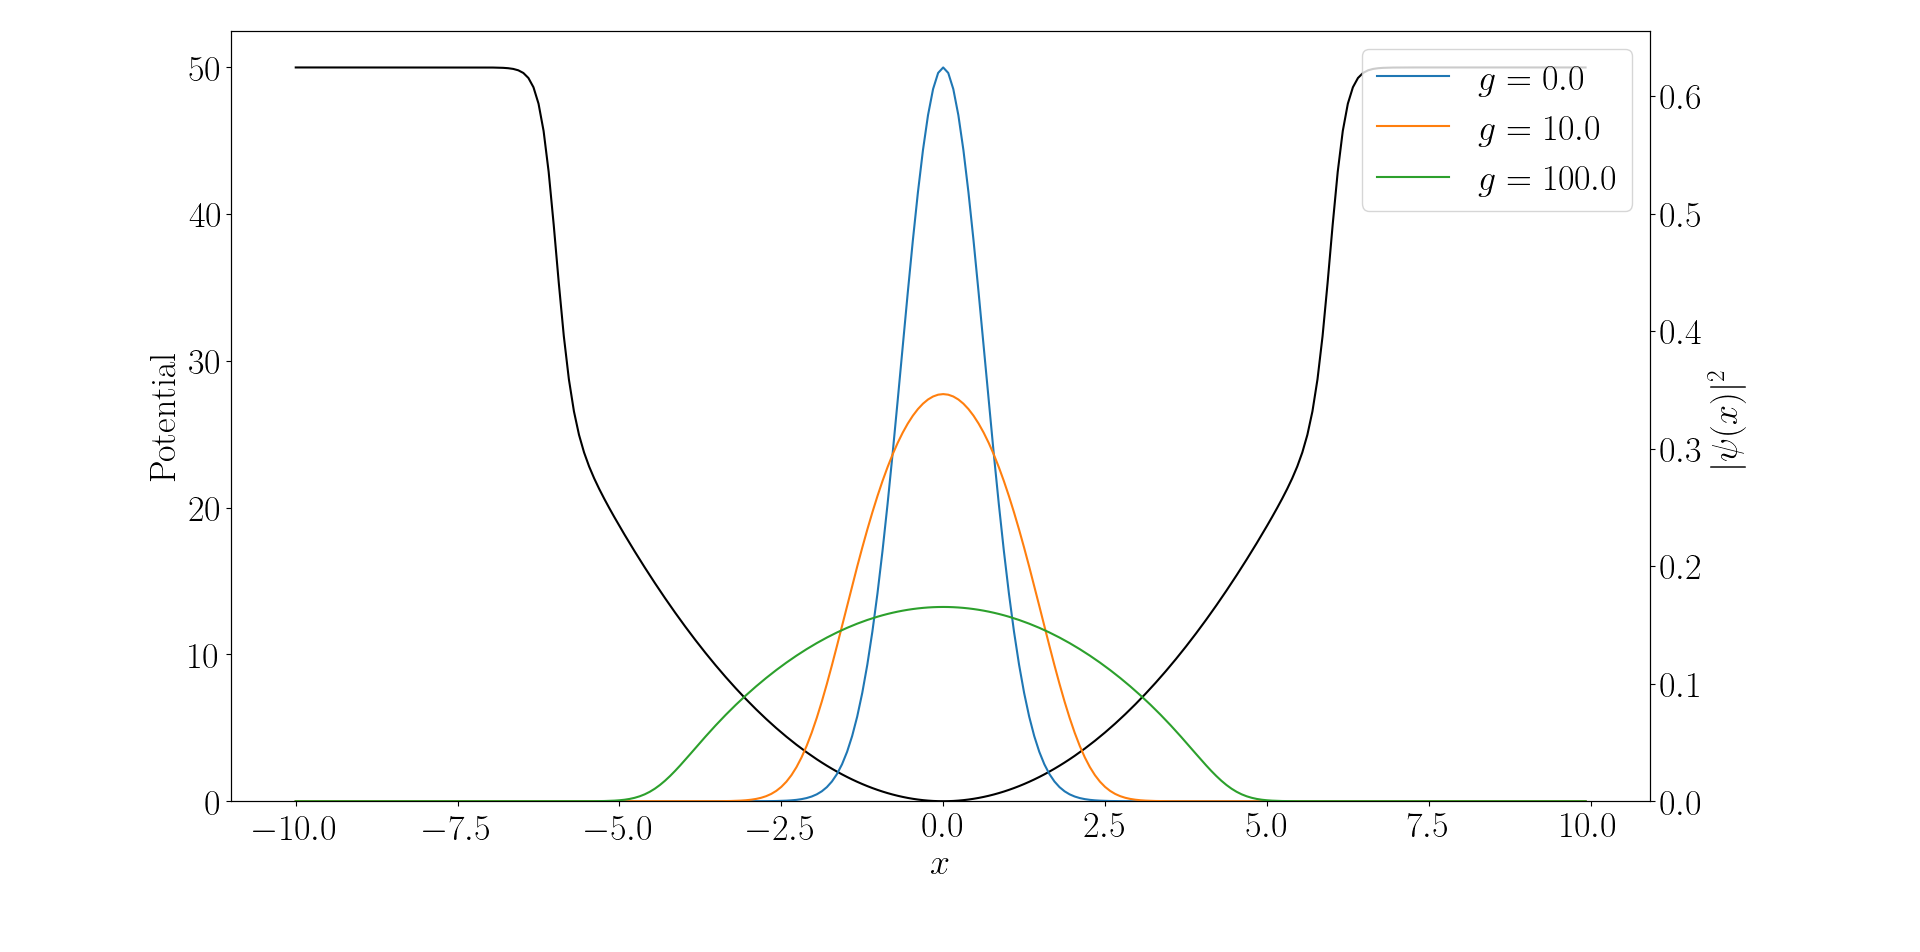
\includegraphics[width=\textwidth]{pot-inter}
\end{column}

\begin{column}{0.2\textwidth}  %%<--- here
    \begin{center}
\begin{figure}[]
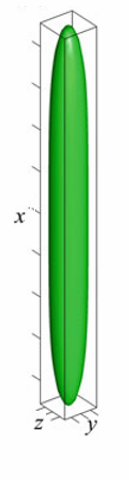
\includegraphics[width=1.3cm]{onedimbose2.png}
\end{figure}
     \end{center}
\end{column}
\end{columns}

\end{frame}

\subsection{Random Potential Generation}

\begin{frame}{Random Potential Generation}

\graphicspath{{"../figs/potentials/"}}
\begin{figure}[H]
    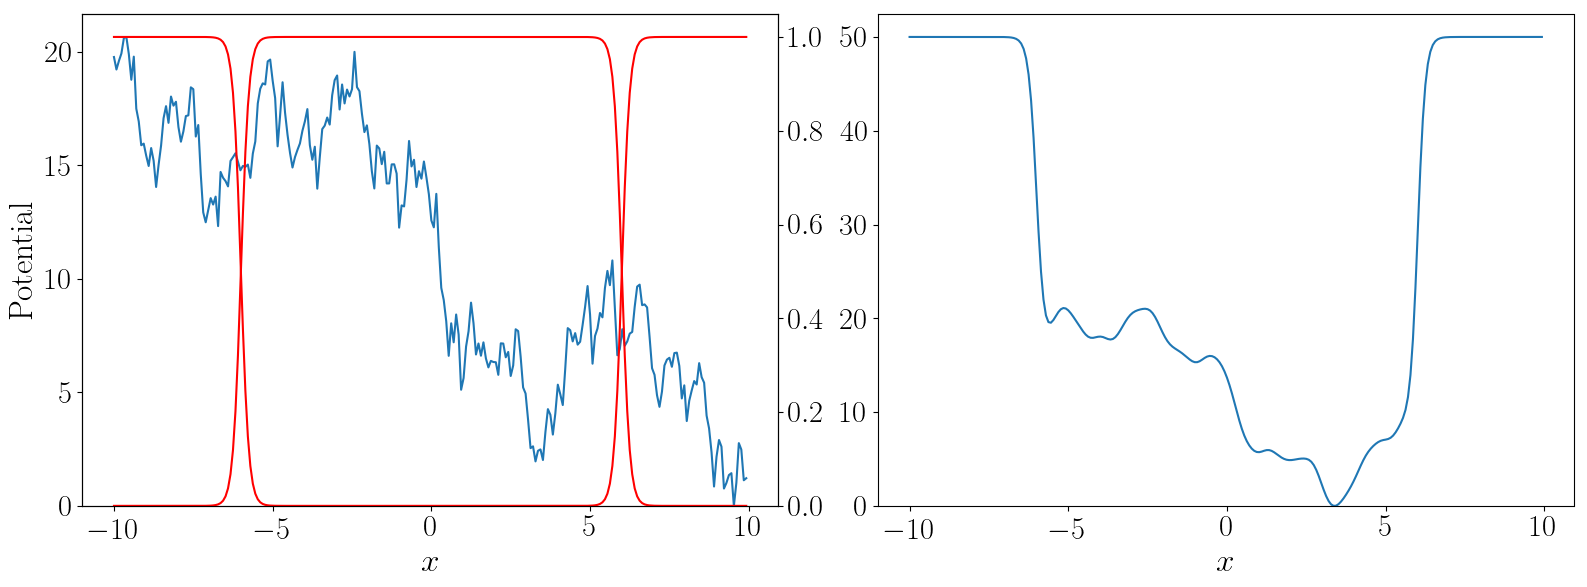
\includegraphics[width=\linewidth]{randombeforeafterproc}
\caption{Envelope functions are applied to a random potential. After that, a gaussian filter is applied for smoothness. We also make sure that the minimum value of the potential is zero at re-scaling process.}
\end{figure}

    
\end{frame}



\begin{frame}{Random Potential Generation}


\graphicspath{{"../figs/potentials/"}}
\begin{figure}[H]
    \centering
    \begin{subfigure}[t]{0.30\textwidth}
        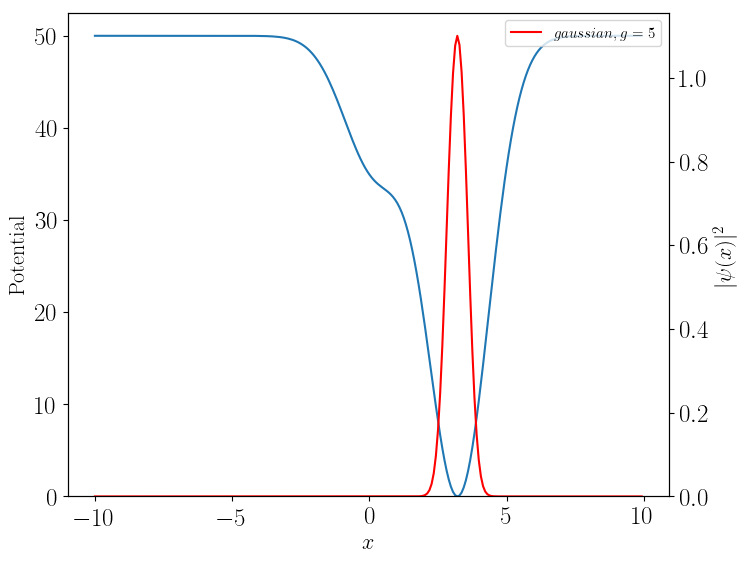
\includegraphics[width=\linewidth]{potvsdensity-gaussian}
        \caption{DIG}
    \end{subfigure}
    \begin{subfigure}[t]{0.30\textwidth}
        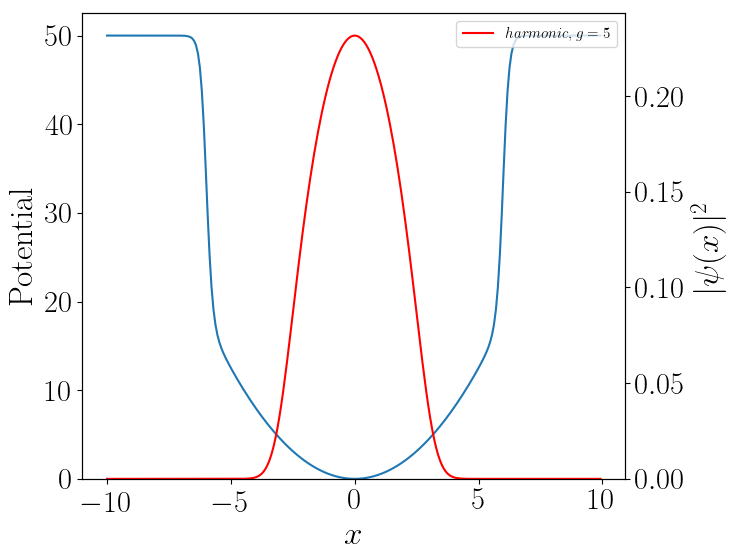
\includegraphics[width=\linewidth]{potvsdensity-harmonic}
        \caption{Harmonic}
    \end{subfigure}
    \begin{subfigure}[t]{0.30\textwidth}
        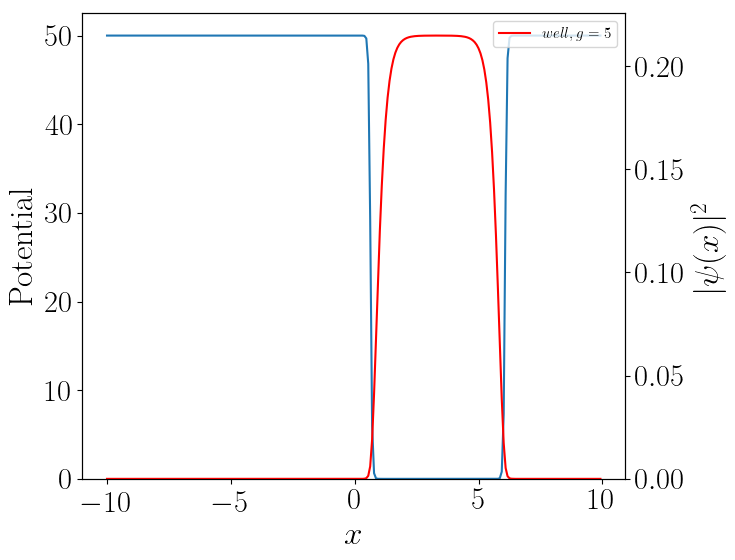
\includegraphics[width=\linewidth]{potvsdensity-well}
        \caption{Well}
    \end{subfigure}
    \begin{subfigure}[t]{0.30\textwidth}
        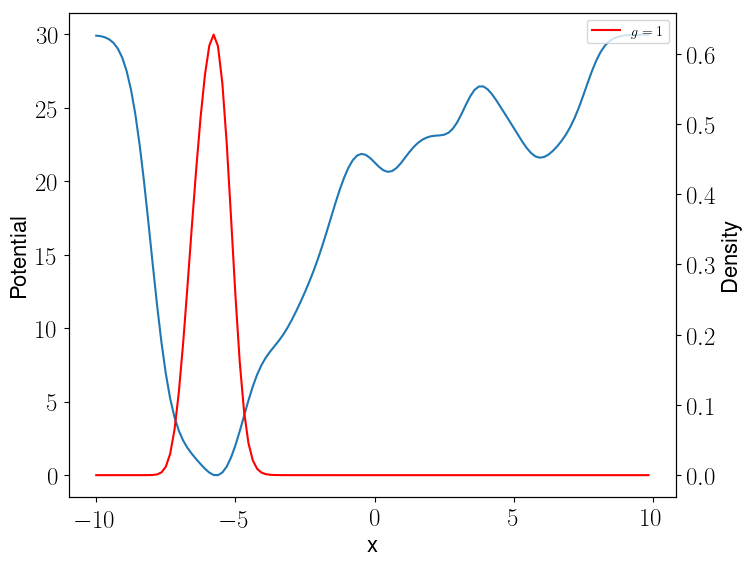
\includegraphics[width=\linewidth]{potvsdensity-random}
        \caption{Random Type 1}
    \end{subfigure}
    \begin{subfigure}[t]{0.30\textwidth}
        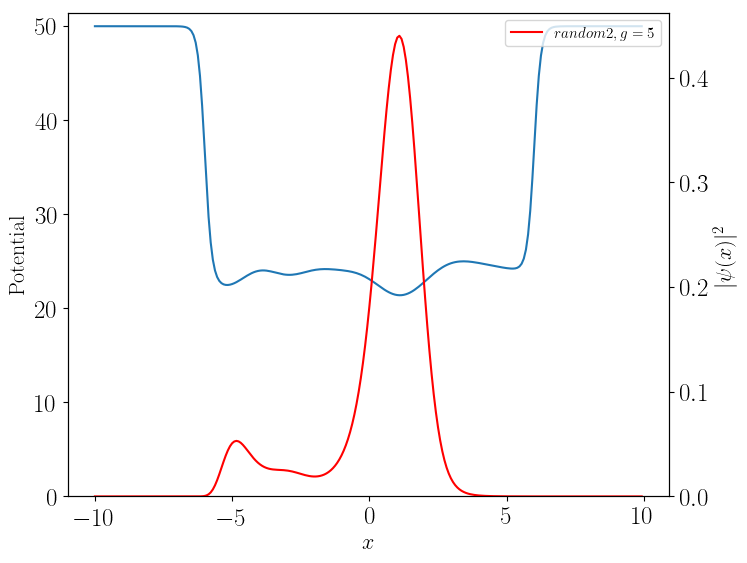
\includegraphics[width=\linewidth]{potvsdensity-random2}
        \caption{Random Type 2}
    \end{subfigure}
    \begin{subfigure}[t]{0.30\textwidth}
        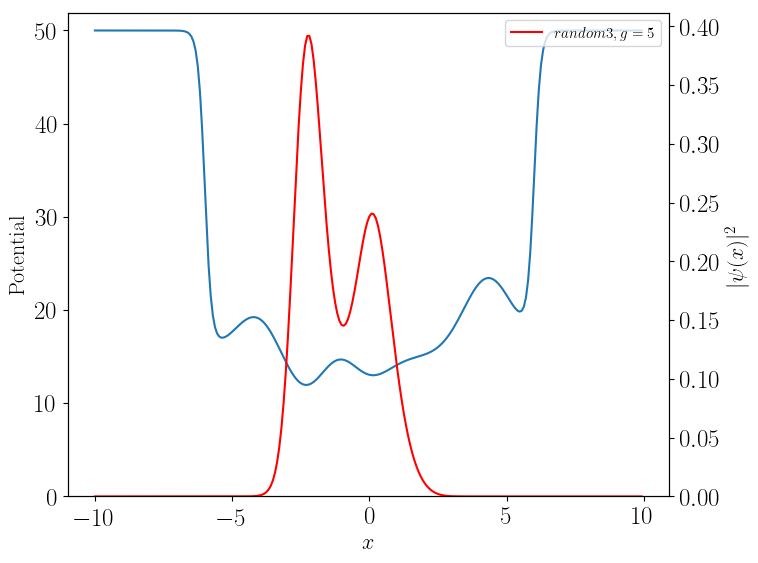
\includegraphics[width=\linewidth]{potvsdensity-random3}
        \caption{Random Type 3}
    \end{subfigure}
\end{figure}
 
\end{frame}

\begin{frame}{Energy Distribution}
    \graphicspath{{"../figs/dataresults/"}}
    \begin{figure}[H]
        \centering
        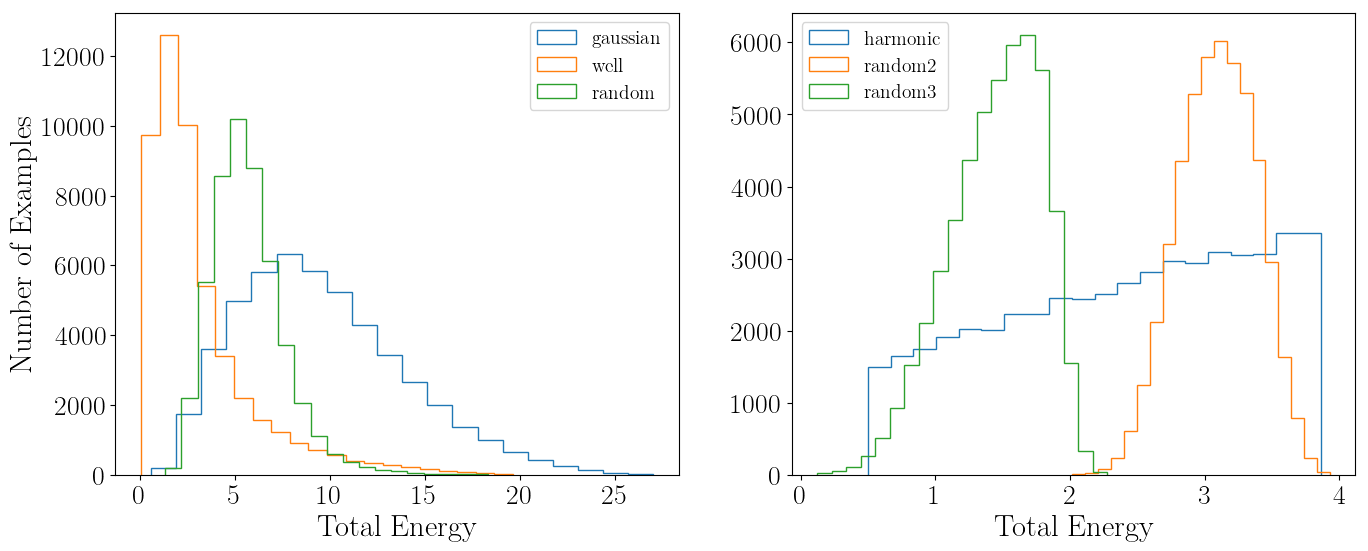
\includegraphics[width=\linewidth]{energydist}
    \caption{The energy distribution of the random potentials are similar but it is clear that the random potential generation method directly affects the energy spectrum. There is a shift between energy spectrum of the random2 and random3. The random's spectrum is completely different and contains both random2's and random3's.}
    \label{fig:energy_dist}
    \end{figure}
\end{frame}

\section{Machine Learning and Differential/Eigenvalue Equations}

\subsection{Machine Learning with Neural Networks}

\begin{frame}{Machine Learning with Neural Networks}

$\bullet$ Artificial neural networks used in machine learning can approximate any continuous function within desired accuracy.
\vskip 1cm

\begin{columns}
\begin{column}{0.40\textwidth}
\hspace*{0.2cm} $\bullet$ It is guaranteed that \hspace*{0.2cm} there exists
a network that \hspace*{0.2cm} satisfies the relation \hspace*{0.2cm} $||\boldsymbol{g}(\boldsymbol{x}) − \boldsymbol{f}(\boldsymbol{x})|| < \epsilon$.
\vskip 1cm
\end{column}
\begin{column}{0.8\textwidth}
    \begin{figure}[Htb!]
        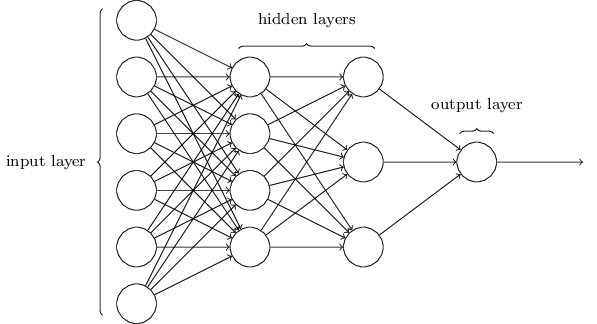
\includegraphics[width=0.6\textwidth]{neuralnetworkex.png}
    \end{figure}
\end{column}
\end{columns}
\vskip 1cm

$\bullet$ Many different kind of applications of machine learning have already been implemented in physics.


\end{frame}

\subsection{Deep Learning and Schr{\"o}dinger Equation}

\begin{frame}{Deep Learning and Schr{\"o}dinger Equation}

$\bullet$ Application of machine learning to a 2D Schr{\"o}dinger Equation with random potential.

\begin{figure}[Htb!]
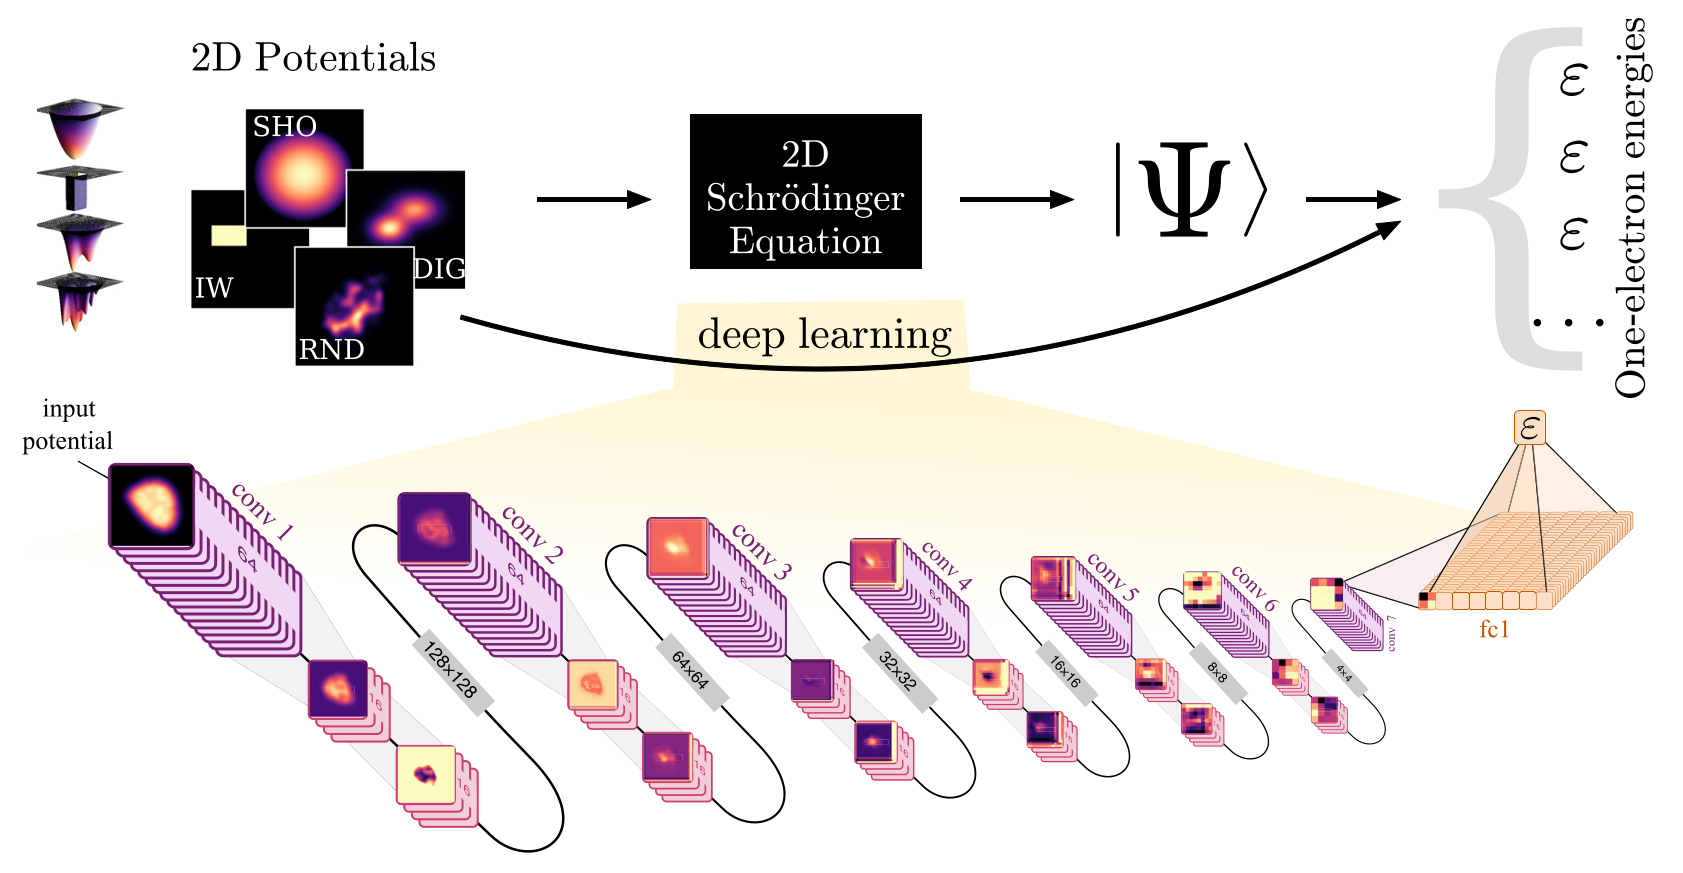
\includegraphics[width=0.8\textwidth]{DPandSE.png}
\caption{\label{fig:DPandSE} Deep Learning and Schr{\"o}dinger Equation.}
\end{figure}

\end{frame}



\section{Convolutional Neural Networks}

\begin{frame}{Convolutional Neural Networks}

\large{\textbf{Convolution Network for Energy Prediction}}: \\
\vskip 0.3cm
$\bullet$ 3 convolution layers, 3 maxpool layers, 3 fully connected layer.
\vskip 0.2cm
$\bullet$ Adaptive Learning Rate (Adam)
\vskip 0.2cm
$\bullet$ ReLU activation function
\vskip 0.5cm


\large{\textbf{Convolution Network for Interaction Parameter}}: \\
\vskip 0.3cm
$\bullet$ 5 convolution layers, 5 maxpool layers, 4 fully connected layer.
\vskip 0.2cm
$\bullet$ Adaptive Learning Rate (Adam)
\vskip 0.2cm
$\bullet$ ReLU activation function



\end{frame}

\section{Results}
\subsection{Ground State Energy Predictions}
\begin{frame}{Ground State Energy Predictions}
\begin{columns}
    \begin{column}{0.4\textwidth}
        \begin{table}[]
            \centering
            \caption{Prediction Errors}
            \begin{tabular}{lll}
            Potential Type & REM (\%) \\
            DIG            & 1.14     \\
            Harmonic       & 0.05     \\
            Infinite Well  & 2.13     \\
            Random \#1     & 2.24     \\
            Random \#2     & 0.55     \\
            Random \#3     & 0.67                    
            \end{tabular} 
        \end{table}
    \end{column}
    \begin{column}{0.8\textwidth}
    \graphicspath{{"../figs/training/"}}
    \begin{figure}[H]
        \begin{subfigure}[t]{0.80\textwidth}
            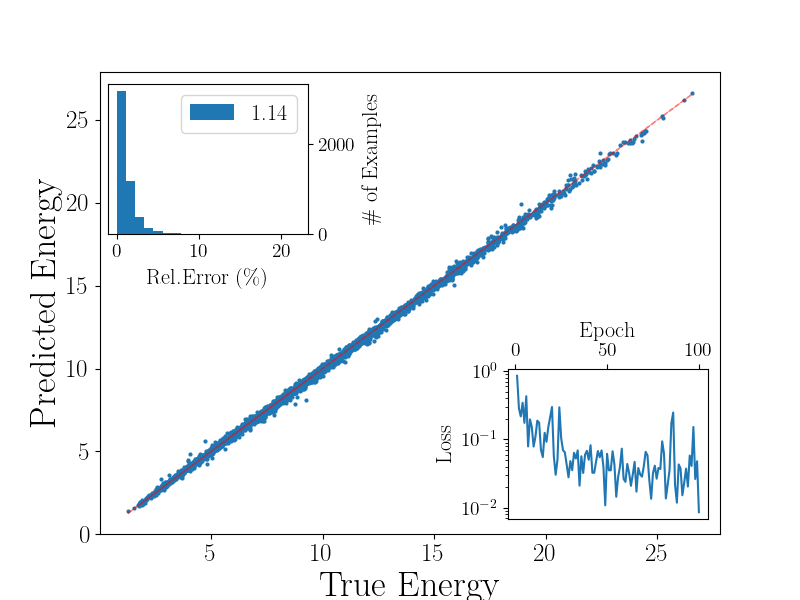
\includegraphics[width=\linewidth]{gaussian}
        \caption{Double Inverted Gaussian}
        \end{subfigure}
    \end{figure}
    \end{column}
\end{columns}
\end{frame}

\begin{frame}{Ground State Energy Predictions}
\begin{columns}
    \begin{column}{0.4\textwidth}
        \begin{table}[]
            \centering
            \caption{Prediction Errors}
            \begin{tabular}{lll}
            Potential Type & REM (\%) \\
            DIG            & 1.14     \\
            Harmonic       & 0.05     \\
            Infinite Well  & 2.13     \\
            Random \#1     & 2.24     \\
            Random \#2     & 0.55     \\
            Random \#3     & 0.67                    
            \end{tabular} 
        \end{table}
    \end{column}
    \begin{column}{0.8\textwidth}
    \graphicspath{{"../figs/training/"}}
    \begin{figure}[H]
        \begin{subfigure}[t]{0.80\textwidth}
            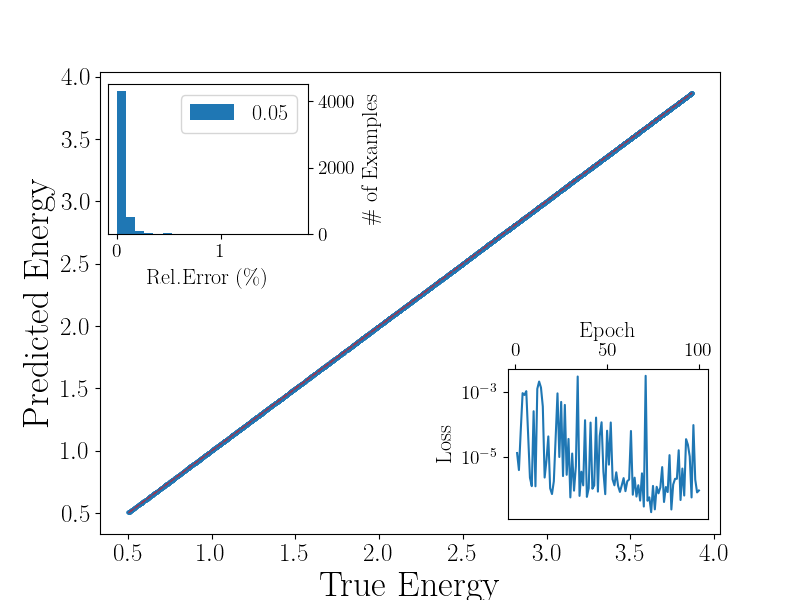
\includegraphics[width=\linewidth]{harmonic}
        \caption{Harmonic}
        \end{subfigure}
    \end{figure}
    \end{column}
\end{columns}
\end{frame}


\begin{frame}{Ground State Energy Predictions}
\begin{columns}
    \begin{column}{0.4\textwidth}
        \begin{table}[]
            \centering
            \caption{Prediction Errors}
            \begin{tabular}{lll}
            Potential Type & REM (\%) \\
            DIG            & 1.14     \\
            Harmonic       & 0.05     \\
            Infinite Well  & 2.13     \\
            Random \#1     & 2.24     \\
            Random \#2     & 0.55     \\
            Random \#3     & 0.67                    
            \end{tabular} 
        \end{table}
    \end{column}
    \begin{column}{0.8\textwidth}
    \graphicspath{{"../figs/training/"}}
    \begin{figure}[H]
        \begin{subfigure}[t]{0.80\textwidth}
            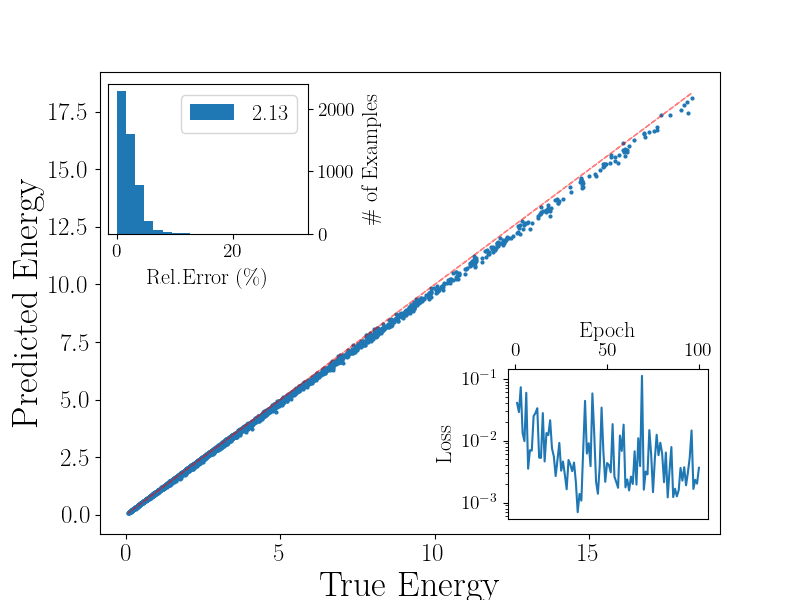
\includegraphics[width=\linewidth]{well}
        \caption{Infinite Well}
        \end{subfigure}
    \end{figure}
    \end{column}
\end{columns}
\end{frame}

\begin{frame}{Ground State Energy Predictions}
\begin{columns}
    \begin{column}{0.4\textwidth}
        \begin{table}[]
            \centering
            \caption{Prediction Errors}
            \begin{tabular}{lll}
            Potential Type & REM (\%) \\
            DIG            & 1.14     \\
            Harmonic       & 0.05     \\
            Infinite Well  & 2.13     \\
            Random \#1     & 2.24     \\
            Random \#2     & 0.55     \\
            Random \#3     & 0.67                    
            \end{tabular} 
        \end{table}
    \end{column}
    \begin{column}{0.8\textwidth}
    \graphicspath{{"../figs/training/"}}
    \begin{figure}[H]
        \begin{subfigure}[t]{0.80\textwidth}
            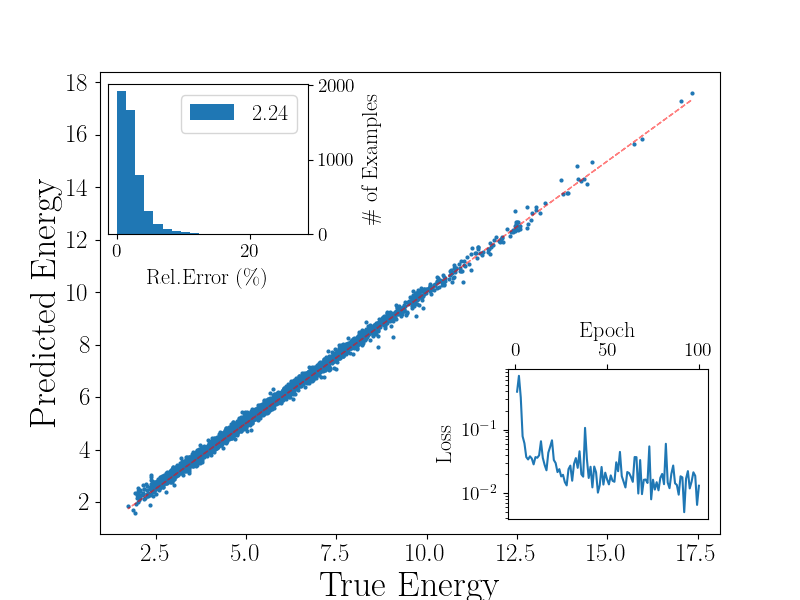
\includegraphics[width=\linewidth]{random}
        \caption{Random Type 1}
        \end{subfigure}
    \end{figure}
    \end{column}
\end{columns}
\end{frame}

\begin{frame}{Ground State Energy Predictions}
\begin{columns}
    \begin{column}{0.4\textwidth}
        \begin{table}[]
            \centering
            \caption{Prediction Errors}
            \begin{tabular}{lll}
            Potential Type & REM (\%) \\
            DIG            & 1.14     \\
            Harmonic       & 0.05     \\
            Infinite Well  & 2.13     \\
            Random \#1     & 2.24     \\
            Random \#2     & 0.55     \\
            Random \#3     & 0.67                    
            \end{tabular} 
        \end{table}
    \end{column}
    \begin{column}{0.8\textwidth}
    \graphicspath{{"../figs/training/"}}
    \begin{figure}[H]
        \begin{subfigure}[t]{0.80\textwidth}
            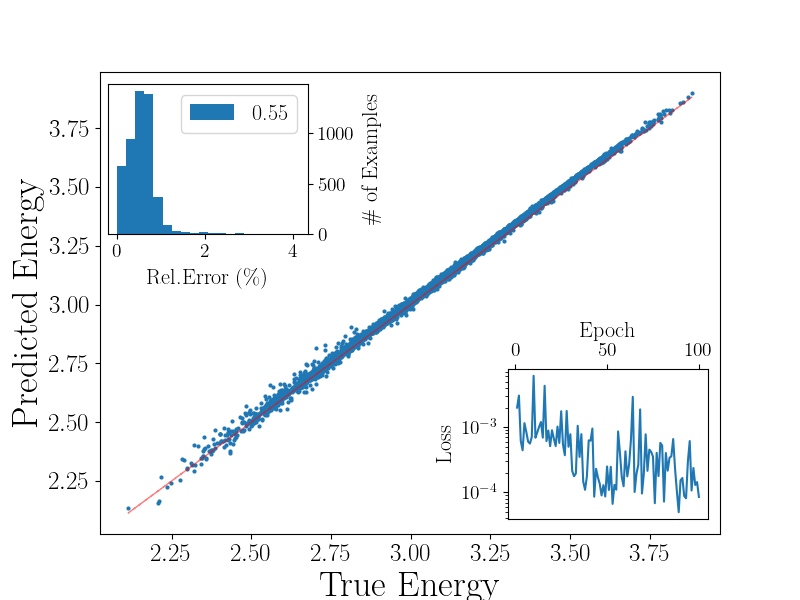
\includegraphics[width=\linewidth]{random2}
        \caption{Random Type 2}
        \end{subfigure}
    \end{figure}
    \end{column}
\end{columns}
\end{frame}

\begin{frame}{Ground State Energy Predictions}
\begin{columns}
    \begin{column}{0.4\textwidth}
        \begin{table}[]
            \centering
            \caption{Prediction Errors}
            \begin{tabular}{lll}
            Potential Type & REM (\%) \\
            DIG            & 1.14     \\
            Harmonic       & 0.05     \\
            Infinite Well  & 2.13     \\
            Random \#1     & 2.24     \\
            Random \#2     & 0.55     \\
            Random \#3     & 0.67                    
            \end{tabular} 
        \end{table}
    \end{column}
    \begin{column}{0.8\textwidth}
    \graphicspath{{"../figs/training/"}}
    \begin{figure}[H]
        \begin{subfigure}[t]{0.80\textwidth}
            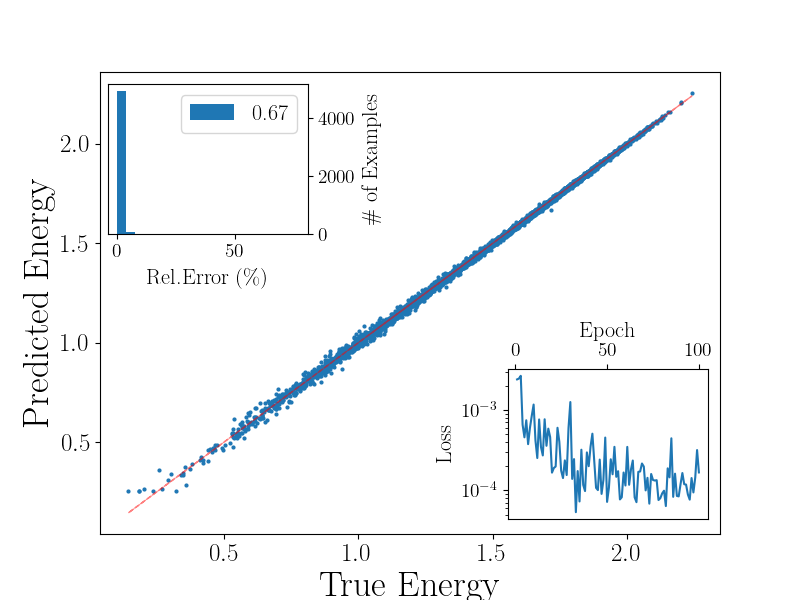
\includegraphics[width=\linewidth]{random3}
        \caption{Random Type 3}
        \end{subfigure}
    \end{figure}
    \end{column}
\end{columns}
\end{frame}

\subsection{Inverse Problem: Interaction Parameter Prediction}
\begin{frame}{Inverse Problem: Interaction Parameter Prediction}
    \begin{columns}
        \begin{column}{0.4\textwidth}
            \begin{table}[]
                \centering
                \caption{Prediction Errors}
                \begin{tabular}{ll}
                    Potential Type & REM (\%) \\
                    DIG            & 1.33     \\
                    Harmonic       & 1.33     \\
                    Infinite Well  & 17.29    \\
                    Random \#1     & 12.77    \\
                    Random \#2     & 10.41    \\
                    Random \#3     & 6.96                    
                \end{tabular}
            \end{table}
        \end{column}
        \begin{column}{0.8\textwidth}
        \graphicspath{{"../figs/training/interaction/"}}
        \begin{figure}[H]
            \begin{subfigure}[t]{0.80\textwidth}
                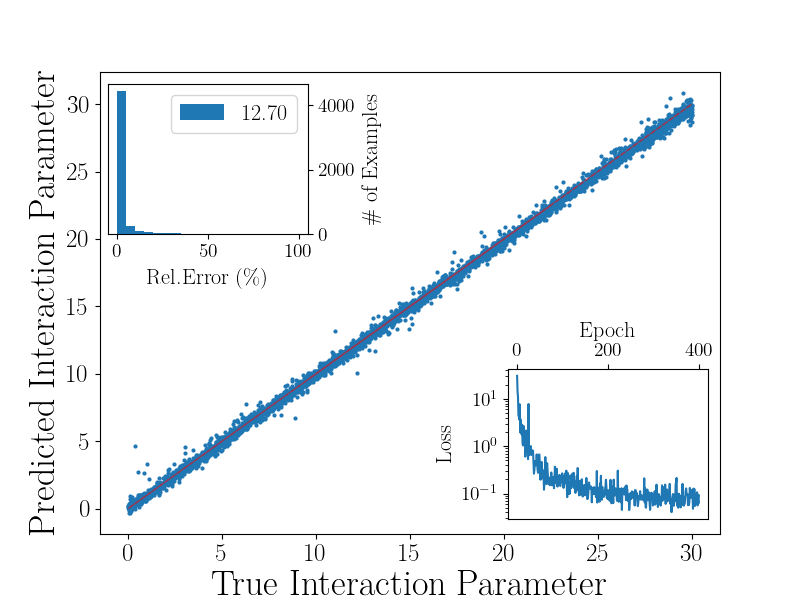
\includegraphics[width=\linewidth]{inter-gaussian}
            \caption{Double Inverted Gaussian}
            \end{subfigure}
        \end{figure}
        \end{column}
    \end{columns}
\end{frame}

\begin{frame}{Inverse Problem: Interaction Parameter Prediction}
    \begin{columns}
        \begin{column}{0.4\textwidth}
            \begin{table}[]
                \centering
                \caption{Prediction Errors}
                \begin{tabular}{ll}
                    Potential Type & REM (\%) \\
                    DIG            & 1.33     \\
                    Harmonic       & 1.33     \\
                    Infinite Well  & 17.29    \\
                    Random \#1     & 12.77    \\
                    Random \#2     & 10.41    \\
                    Random \#3     & 6.96                    
                \end{tabular}
            \end{table}
        \end{column}
        \begin{column}{0.8\textwidth}
        \graphicspath{{"../figs/training/interaction/"}}
        \begin{figure}[H]
            \begin{subfigure}[t]{0.80\textwidth}
                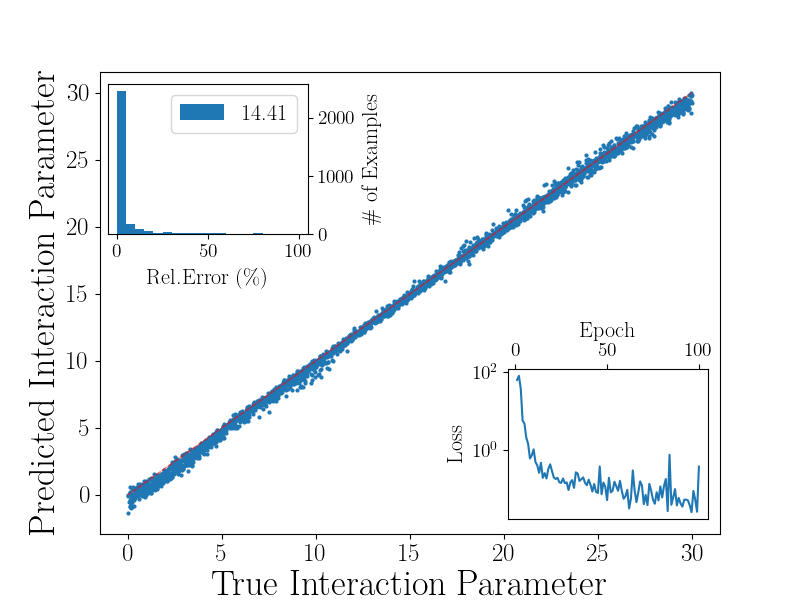
\includegraphics[width=\linewidth]{inter-harmonic}
            \caption{Harmonic}
            \end{subfigure}
        \end{figure}
        \end{column}
    \end{columns}
\end{frame}

\begin{frame}{Inverse Problem: Interaction Parameter Prediction}
    \begin{columns}
        \begin{column}{0.4\textwidth}
            \begin{table}[]
                \centering
                \caption{Prediction Errors}
                \begin{tabular}{ll}
                    Potential Type & REM (\%) \\
                    DIG            & 1.33     \\
                    Harmonic       & 1.33     \\
                    Infinite Well  & 17.29    \\
                    Random \#1     & 12.77    \\
                    Random \#2     & 10.41    \\
                    Random \#3     & 6.96                    
                \end{tabular}
            \end{table}
        \end{column}
        \begin{column}{0.8\textwidth}
        \graphicspath{{"../figs/training/interaction/"}}
        \begin{figure}[H]
            \begin{subfigure}[t]{0.80\textwidth}
                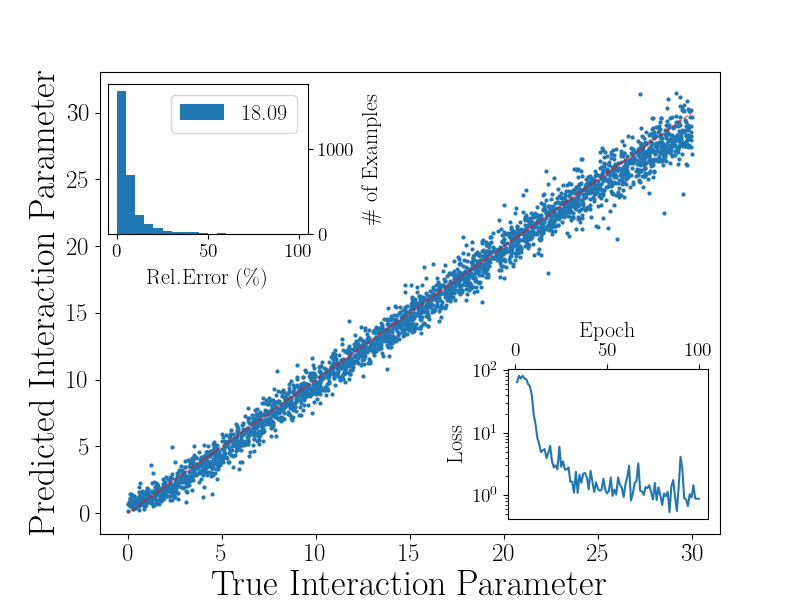
\includegraphics[width=\linewidth]{inter-well}
            \caption{Infinite Well}
            \end{subfigure}
        \end{figure}
        \end{column}
    \end{columns}
\end{frame}

\begin{frame}{Inverse Problem: Interaction Parameter Prediction}
    \begin{columns}
        \begin{column}{0.4\textwidth}
            \begin{table}[]
                \centering
                \caption{Prediction Errors}
                \begin{tabular}{ll}
                    Potential Type & REM (\%) \\
                    DIG            & 1.33     \\
                    Harmonic       & 1.33     \\
                    Infinite Well  & 17.29    \\
                    Random \#1     & 12.77    \\
                    Random \#2     & 10.41    \\
                    Random \#3     & 6.96                    
                \end{tabular}
            \end{table}
        \end{column}
        \begin{column}{0.8\textwidth}
        \graphicspath{{"../figs/training/interaction/"}}
        \begin{figure}[H]
            \begin{subfigure}[t]{0.80\textwidth}
                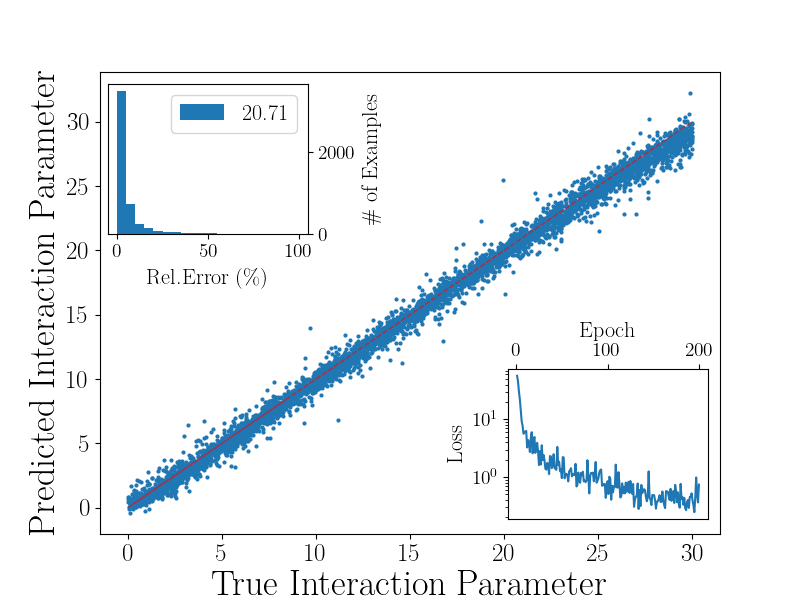
\includegraphics[width=\linewidth]{inter-random}
            \caption{Random Type 1}
            \end{subfigure}
        \end{figure}
        \end{column}
    \end{columns}
\end{frame}


\begin{frame}{Inverse Problem: Interaction Parameter Prediction}
    \begin{columns}
        \begin{column}{0.4\textwidth}
            \begin{table}[]
                \centering
                \caption{Prediction Errors}
                \begin{tabular}{ll}
                    Potential Type & REM (\%) \\
                    DIG            & 1.33     \\
                    Harmonic       & 1.33     \\
                    Infinite Well  & 17.29    \\
                    Random \#1     & 12.77    \\
                    Random \#2     & 10.41    \\
                    Random \#3     & 6.96                    
                \end{tabular}
            \end{table}
        \end{column}
        \begin{column}{0.8\textwidth}
        \graphicspath{{"../figs/training/interaction/"}}
        \begin{figure}[H]
            \begin{subfigure}[t]{0.80\textwidth}
                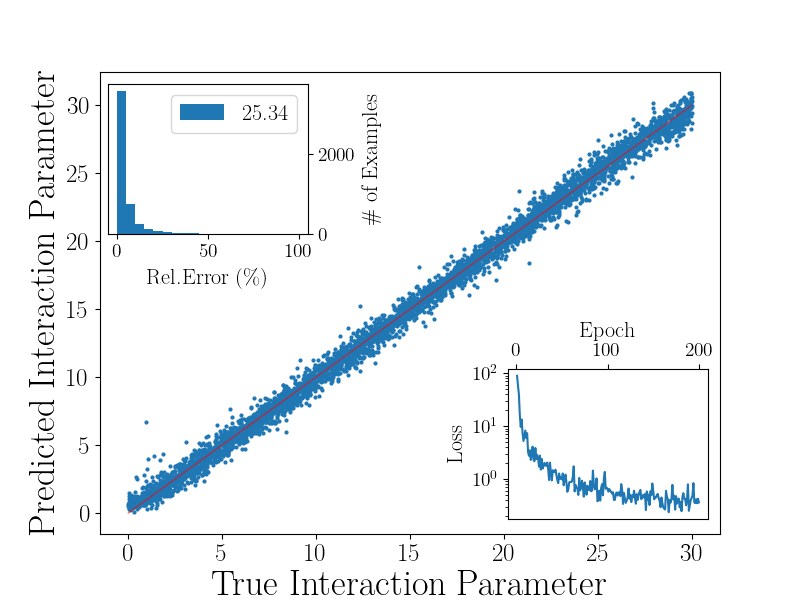
\includegraphics[width=\linewidth]{inter-random2}
            \caption{Random Type 2}
            \end{subfigure}
        \end{figure}
        \end{column}
    \end{columns}
\end{frame}

\begin{frame}{Inverse Problem: Interaction Parameter Prediction}
    \begin{columns}
        \begin{column}{0.4\textwidth}
            \begin{table}[]
                \centering
                \caption{Prediction Errors}
                \begin{tabular}{ll}
                    Potential Type & REM (\%) \\
                    DIG            & 1.33     \\
                    Harmonic       & 1.33     \\
                    Infinite Well  & 17.29    \\
                    Random \#1     & 12.77    \\
                    Random \#2     & 10.41    \\
                    Random \#3     & 6.96                    
                \end{tabular}
            \end{table}
        \end{column}
        \begin{column}{0.8\textwidth}
        \graphicspath{{"../figs/training/interaction/"}}
        \begin{figure}[H]
            \begin{subfigure}[t]{0.80\textwidth}
                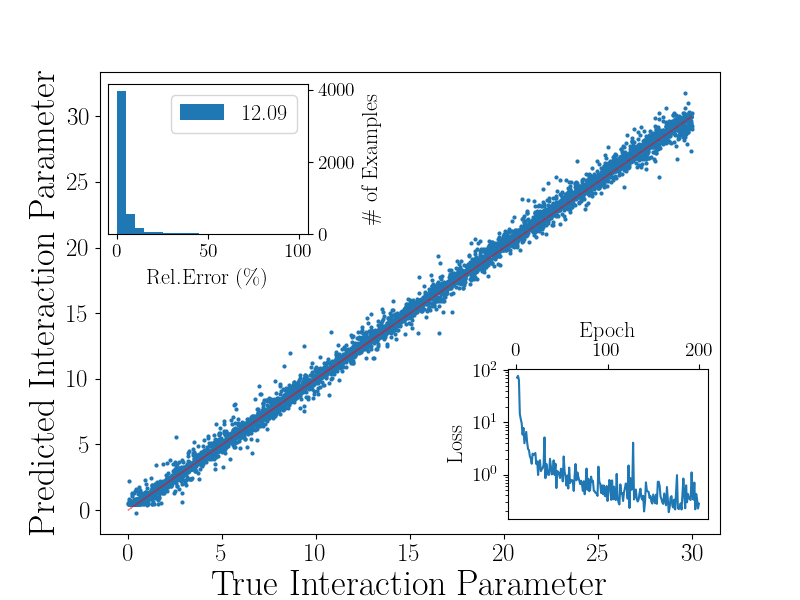
\includegraphics[width=\linewidth]{inter-random3}
            \caption{Random Type 3}
            \end{subfigure}
        \end{figure}
        \end{column}
    \end{columns}
\end{frame}


\section{Conclusion and Future Plans}
\begin{frame}{Conclusion and Future Plan}

\begin{enumerate}
\item Conclusion
    \begin{enumerate}
    \item Machine learning techniques can also be applied to non-linear Schrödinger Equation 
    \item Random potential generation techniques affects the results due to corresponding energy spectrum and distribution.
    \end{enumerate}
\item Future Work
    \begin{enumerate}
    \item Generating uniformly distributed dataset by using variational and approximation methods.
    \item Working in 2D.
    \end{enumerate}
\end{enumerate}



\end{frame}

\end{document}


